\chapter{Application context}\label{chp:2}

\minitoc

\clearpage

The most recent political answer brought to tackle environmental issues in Europe took form under the European Partnership for the Assesment of Risks from Chemicals (PARC) \cite{PARC}. This partnership involves 28 different countries. This new project received a favourable assessment by the European Commission in January 2022 and has started on the 1st of May 2022. The main objectives of PARC are to promote European cooperation, to advance research, to increase knowledge about the risk assessment of chemicals and to train the corresponding methodological skills. Close cooperation between authorities and research will facilitate the translation of research results into regulatory practice. \\
The French Agency for Food, Environmental and Occupational Health and Safety (ANSES) is not only the main French actor in this partnership, but also the coordinator of the entire partnership. This work was funded by the ANSES and aims to support the agency in its mission on French territory. This chapter describes the overall context and the specific problems arising from the characteristics of the data used. The chapter is organized as follows: In \ref{chp:2:1} we introduce ANSES, in \ref{chp:2:2} we detail the task of pesticide monitoring, in \ref{chp:2:3} we focus on the characteristics of pesticide measures, in \ref{chp:2:4} we describe other sources of information of interest, and in \ref{chp:2:5} we define the objectives sought.    

\section{ANSES presentation}\label{chp:2:1}

The ANSES was created in 2010 from the fusion of the French Food Safety Agency (AFSSA) and the French Agency for Environmental and Occupational Health Safety (AFSSET). It is a public administrative body reporting to the Ministries of Health, the Environment, Agriculture, Labour and Consumer Affairs.  

\subsection{Missions} 

\begin{itemize}
\item \textbf{Research activities:} the agency contributes to the progress of new scientific knowledge on the exposure of humans, animals, plants, and the environment to various hazards and risks and is tasked with improving their surveillance. Research topics focus on three areas: animal health and welfare, plant health, and food safety. ANSES is also involved in the development of new analytical methods and detection techniques to identify pathogens and contaminants, whether in the natural environment or in the production chain. This mission also regroups the activities health monitoring and alert. The agency takes part in epidemiological surveillance platforms on animal health, plants health and food chain safety. This mission also tasks ANSES to coordinate five different monitoring systems that covers the following areas: toxicovigilance, surveillance on food supplements, phytopharmacovigilance which will be further investigated in \ref{chp:2:2}, vetenary pharmacovigilance and surveillance and prevention of professionnal pathologies.      
\item \textbf{Risk assessment:} ANSES responds to society's questions about potential risks arising from the consumption of food, the use of certain products or technologies, professionnal activities, or pollution of various environmental compartments (e.g., air, water, or soil). Given the complex risks, the agency has developed a working methodology that brings together many disciplines to provide the most complete response possible. The risk and efficacy assessment of veterinary medicines and phytopharmaceutical products for human and animal health and the environment also falls within the agency's remit. The goal is to define management measures to handle such risks. In particular, ANSES is responsible for granting marketing authorizations for such products and thus also has the authority to withdraw products at the national level \cite{ansesdec}. 
\item \textbf{Public and environmental protection:} ANSES makes recommendations to support public debates and decisions. Its activities contribute to the implementation of effective preventive and protective measures on various societal issues such as health, biodiversity, and ethics. It also provides public access to reliable, independent, and multidisciplinary scientific information. The agency's role is to respond flexibly to already known or emerging, short- or long-term sanitary risks. In other words, the goal is to identify and make recommendations on all emerging signals as quickly as possible, even in times of crisis with scientific uncertainty. The task is then to reduce the degree of uncertainty when possible. Recommendations are based on all available knowledge, whether it was generated by the agency itself or by its partners. 
\end{itemize}

\subsection{Means of action}

The ANSES has the means to carry out and fund research in conjunction with the French and international scientific communities. It has 9 laboratories distributed among its 16 sites on French territory (including overseas departments). The research carried out in these facilities deals with the complex interactions between the environment, human health and animal health. The aim is to anticipate the emergence of zoonosis or animal diseases that could have an economic impact and to combat antibiotic resistance. In detail, the main directions of this research are:
\begin{itemize}
\item learning the characteristics of pathogens (such as fungi, bacteria, viruses or parasites), macroorganisms (such as insect pests or invasive plants) and chemical contaminants. 
\item detect them using state-of-the-art analytical methods.
\item monitor them using powerful epidemiological methods.
\item understand the impact of animal husbandry on animal welfare and health.
\item develop useful knowledge for the development of new treatments and vaccines to prevent and control animal and plant diseases. 
\end{itemize} 
The 9 laboratories have been designated as reference laboratories for pathogen research under more than 100 national and international mandates \cite{ANSESLABS}.

In addition to its research activities, the ANSES is also at the center of a network of partners. Given the scope of the areas it covers, the agency does not have the resources to collect data on all the topics it is asked to address. Therefore, for each topic, it conducts discussions with other organizations that are likely to provide interesting sources of information. For example, each monitoring system coordinated by the agency mobilizes a different set of partners. We will see the different datasets that those partners bring in sections \ref{chp:2:3} ans \ref{chp:2:4}. 

\subsection{Specific organisation}

Many national agencies are counterparts of ANSES. They all participate in the PARC partnership. Each shares data collected at the national level, enabling research studies at the European level. However, each agency is dependent on the network that collected the data it stores and on the internal policies of the country to which it belongs. This leads to heterogeneity on different topics and at different levels. \\
For example, internal policies influence the list of monitored products, and some substances are not studied in certain countries because they are not even approved for sale. This leads to a patchwork of different susbtances lists at the European level as shown in \cite{Baran2022}. Some heterogeneity is also observed at the national level. For example, in France, it was determined that drinking water quality data should be collected at the regional level \cite{Baran2022}. Each regional agency is responsible for the quality of the data it shares with ANSES. We will see the impact of this organisation on the data in \ref{chp:2:3}. \\
Thus, the structure of the monitoring system is country-specific. This is especially true for the pesticides monitoring system, on which we will focus on below.

\section{Pesticides monitoring mission}\label{chp:2:2}

Although the term risk is often confused with hazard in common usage, they do not have the same definition. A \textbf{health hazard} is the inherent ability of a substance or organism to cause adverse health effects. \textbf{Exposure} is the specific situation in which people are confronted with a health hazard. Exposure can be characterized by the following questions:
\begin{itemize}
\item what was the degree or intensity of exposure?
\item how long and how regularly does the exposure occur? 
\item in what manner does the exposure occur? (Is it skin contact, ingestion?). 
\end{itemize}
A \textbf{health risk} occurs when one is exposed to a health hazard. It is defined as the probability of the occurrence of adverse effects on human health. It can take many forms, such as infection, poisoning, or chronic disease (such as diabete or asthma). The outcome depends on the characteristics of the exposure and the characteristics (like age or immunity) of the animal, human or plant population under study.

ANSES is tasked with studying and monitoring health risks caused by various factors. In particular, the agency is charged with monitoring health risks associated with chemical agents. The pesticide surveillance mission can be formally defined as a surveillance system that collects and evaluates monitoring data on phytopharmaceuticals (pesticides). It can also be referred to as phytopharmacovigilance. The aim is to detect adverse effects associated with the use of these products as soon as possible in order to protect the health of living organisms and ecosystems. Pesticide health hazards are well referenced by the Agency and available in the AGRITOX database. Different types of exposures can be distinguished depending on the population affected by the monitoring. We give two different specific cases of exposures with different populations. The first case is about monitoring the health risk of professional farmers. They are regularly exposed to pesticides that they apply. The exposure is then long-term and the likely routes by which they could come into contact with the substance would be inhalation or dermal contact. The second case involves monitoring the health risk to aquatic fauna. Exposure to pesticides may result from the effects of water runoff following pesticide application, which could lead to dispersal into the river system in the area. Since the pesticide is in the same environment as the aquatic fauna, it could come into direct contact with them and cause adverse effects (acute or chronic). It should be noted that diffusion, and thus exposure, depends on external factors, independent of the intrinsic properties of the substance. One example would be meteorological conditions during the study period. Another example would be to consider the environmental characteristics that are likely to influence the diffusion of the substance. For example, the diffusion of a chemical product in a river system might be influenced by the riverbed composition or the width of the river. Identifying regions where those characteristics are fixed would be idea for studying the exposure, the hydro-ecoregions (HER) provide a good took to work with in the river system example.           

Anses does not itself collect the data it needs to fulfil its phytoharmacovigilance mission. It relies on its partner network to obtain data sets of interest. The decision to add a new source of information first requires a discussion of the coherence of the use of that source of information to provide an answer to the problem under study. For phytopharmacovigilance, the following information is of interest: 
\begin{enumerate}
\item contamination of the environment - air, water, soil, food and drinking water - by residues including metabolites of pesticides.
\item exposure, impregnation and effects on living organisms and ecosystems as a whole: humans, livestock and wildlife, crops, flora, etc. Resistance phenomena in organisms targeted by these molecules: Pathogens, weeds, insects.
\end{enumerate}
This results in collecting spatio-temporal informations. The data sets that provide information on pesticide concentrations and use are presented in detail in section \ref{chp:2:3}.

\section{Pesticides measurments data}\label{chp:2:3}

There are two types of measurements: direct measurements, which are essentially stations that measure the exact concentration of a substance in a particular environment, and indirect measurements, which give indications of the use of a substance.

\subsection{Direct measurments characteristics}

In this part, the characteristics of pesticides direct measures from sampling stations are studied. The following characteristics are not found systematically, but are very common when it comes to concentration measurements.

\subsubsection{Chemical precision limits in measurments}

The first specificity of concentration measurement arises from the problem of measuring a chemical substance in a sample. In applied chemistry, any measuring device is characterized by two types of limits. 

\begin{itemize}
    \item the detection limit (LOD): This is the smallest concentration value in a sample that can be distinguished from zero with certainty.
    \item the limit of quantification (LOQ): This is the smallest concentration value of a substance in a sample that can be measured with certainty. 
\end{itemize}

These limits are determined by the sensors that the sampling station is equiped with. It happens that geographical areas are covered by stations that do not have the same equipment. In this case, there are several LOQ values within the samples taken in that area. In the case of surface waters, for example, the contracts for the selection of monitoring laboratories are awarded by the water agencies. These agencies, six in number, cover an area larger than the French administrative regions. This means that if the scale of an administrative region is taken as the basis for a study, this region may fall under the jurisdiction of two different water agencies and therefore the measuring instruments may be different. Moreover, the same station may change its measuring equipment over time. Station equipment contracts are renewed periodically, but renewal does not guarantee that the same equipment will be maintained. All those caracteristics are illustrated in Figure \ref{fig:cens_ex}. These two limits of accuracy mean that concentration data are left-censored. In Chapter 4, we will show which method was chosen to handle this type of data in this thesis. Several methods have been developed to handle this type of data. We can cite the imputation of values to replace the LOQ values present in the set of concentration values, the use of the maximum likelihood estimator or the Kaplan-Meier estimator (see \cite{Gillaizeau2020,Croghan2003MethodsOD}). 

\begin{figure}
    \centering
    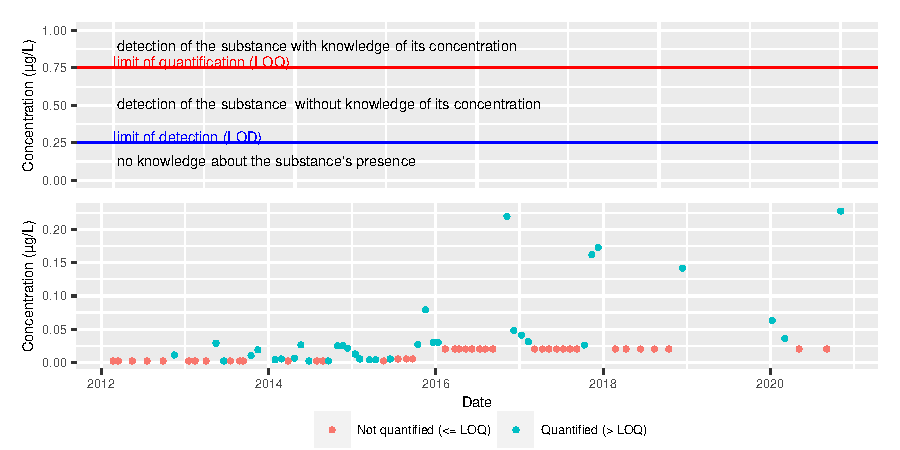
\includegraphics{Chap3/Cens_ex.pdf}
    \caption{Censorship illustration. The top Figure sums up the limits of measurements effects. The bottom Figure shows the consequences of censorship on the samples of a station located in the Centre-Val de Loire region. This station changed its equipment in 2016, the LOQ change values.}
    \label{fig:cens_ex}
\end{figure}

\subsubsection{Irregular sampling}

The second feature is a direct consequence of Section \ref{chp:2:1}. We mentioned that each country has organised its own monitoring system. Some features are country specific and have an impact on the raw data of the collected samples. Sampling in France is not necessarily done at regular intervals, as can be seen in Figure \ref{fig:cens_ex}. No sample was made during the year 2019. This is also true for water monitoring data. This is a peculiarity of the French network, as this is not the case in all countries. For example, \cite{Zhang2008} states that sampling in surface waters is regular in China. Furthermore, \cite{Joergensen2008} states that this is also the case for groundwater monitoring systems in countries such as China, the Netherlands, and South Korea. The South Korean monitoring system is even automatic, and a sample is taken every six hours and automatically stored on a central server after analysis. We would also like to point out that strategies other than regular sampling, such as grab sampling \cite{Novic2017} could explain the irregular sampling rythm in French surface water quality. Grab sampling consists of obtaining as accurate a picture as possible of surface water quality in a short period of time (and in a limited area). If the operations of grab samples and periodic monitoring operations of a station are reported in the same database, irregular sampling may also occur.  

\subsubsection{Spatio-temporal heterogeneity}

Another main chgaracteristics mentionned in \cite{Baran2022} is the spatio-temporal heterogeneity in the data-sets. Figure \ref{fig:het_samp_ex} shows the temporal heterogeneity. For two spatially neighbouring stations the measured values are not synchronous in time. It can also be seen that the stations take very few measurements and do not take the same number of measurements. In Figure \ref{fig:het_samp_ex} we see that it is not possible to compare the measurements of the two existing stations. The stations made samples in non-overlapping time periods. One may notice that aggregating the data from the two stations results in a time series that is more evenly sampled over time. More details on this issue are provided in Section \ref{chp:2:4}. 

\begin{figure}[ht]
    \centering
    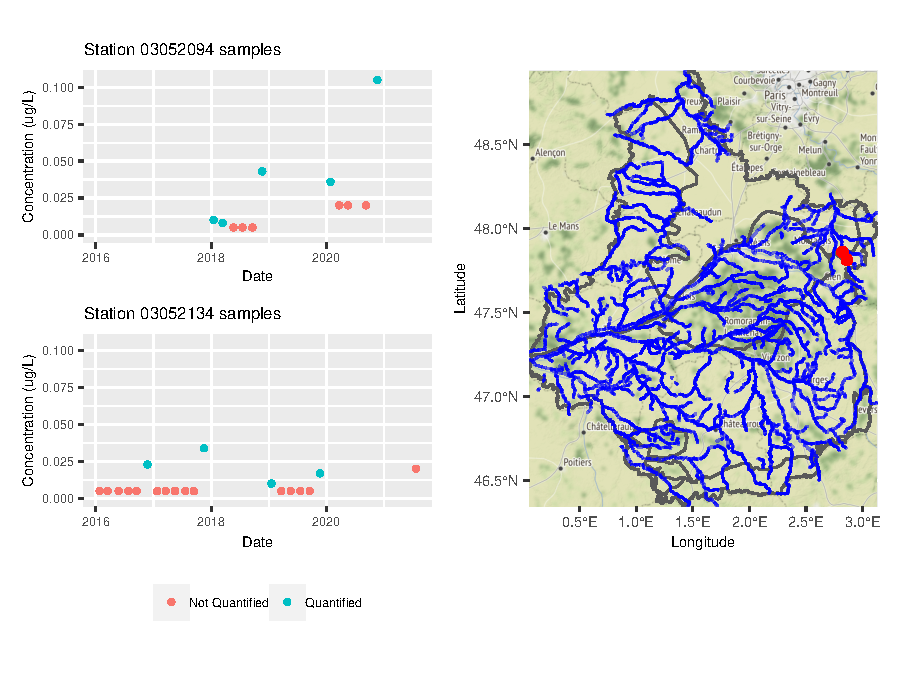
\includegraphics{Chap3/Hetero_ex.pdf}
    \caption{Spatial and temporal heterogeneity in sampling. The Figures on the left represent all the samples of two neighbouring stations. The map on the right shows the position of those stations.}
    \label{fig:het_samp_ex}
\end{figure}

Figure \ref{fig:het_spa_ex} illustrates that alongside temporal heterogeneity induced by the stations different sampling rhythms, spatio temporal data are not distributed in a homogeneous way over the territory. The concentrations value seem to completely differ according to their spatial area of origin. Thus, the data are heterogeneous in space. Figure \ref{fig:het_spa_ex} also illustrates that the distribution of concentration values can drastically change over time. Looking at the samples of station 03189000, there is a break point just before the year 2015 in the station concentration values. The same can be said for the year 2016 in Figure \ref{fig:cens_ex}. Thus the data are heterogeneous in space and in time.  

\begin{figure}[ht]
    \centering
    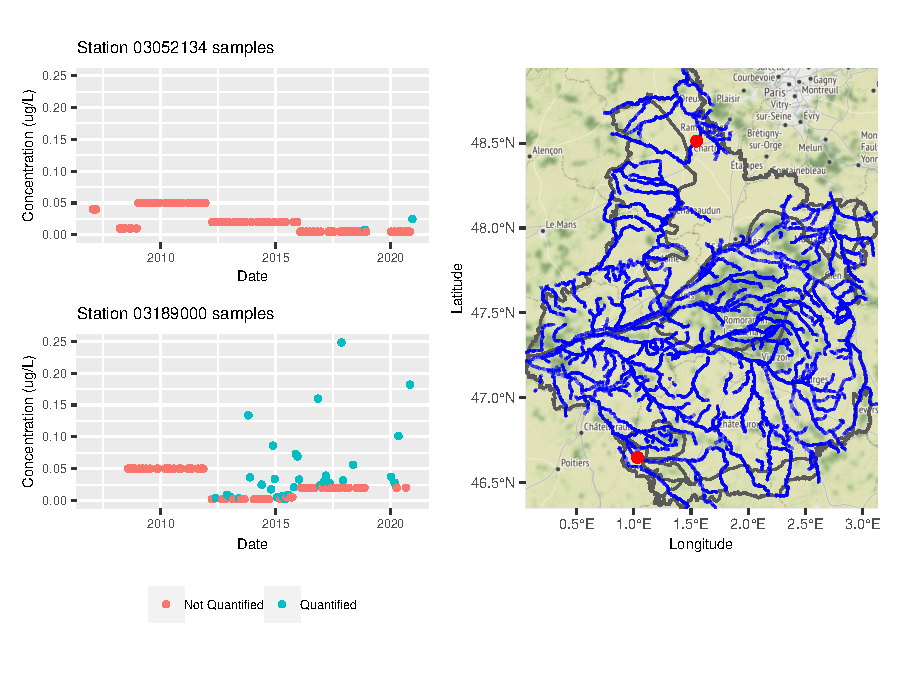
\includegraphics{Chap3/het_spa_ex.pdf}
    \caption{Spatial and temporal heterogeneity in distribution. The Figures on the left represent all the samples of two stations. The map on the right shows the position of those stations.}
    \label{fig:het_spa_ex}
\end{figure}

\subsection{Indirect measurments information}

\subsubsection{Surveys on farming pratices}

Additional clues to the substance presence can be obtained from surveys of agricultural practices. They are conducted in the form of a questionnaire and are used to describe and characterize how farmers operate on their land. These studies are very specific and focus only on certain types of crops. Three topics are addressed in the questionnaires. The first captures general information about the farm, such as commitment to pesticide use reduction or agroecology. The second questionnaire is designed to capture all technical operations on the farm plot. In other words, we examine the structure of the plantation, its preceding crops or its irrigation. Finally, the use of pesticides on the whole farm is studied. The questionnaire goes over criterias such as the type and settings of the sprayer for the substance or the handling and protection of the user.  
Figure \ref{fig:PK1} shows what kind of questions to expect in this survey\footnote{Document in French, full document in \cite{PK}}. In summary, farming practice surveys provide much qualitative (rather than quantitative) information about the source of substance emissions. However, these surveys are conducted on an ad hoc basis and cover only certain types of crops. Only the results of the statistical departments of Agricultural ministry analyses \cite{PK2} are available however the raw data is not. 

\begin{figure}[ht]
    \centering
    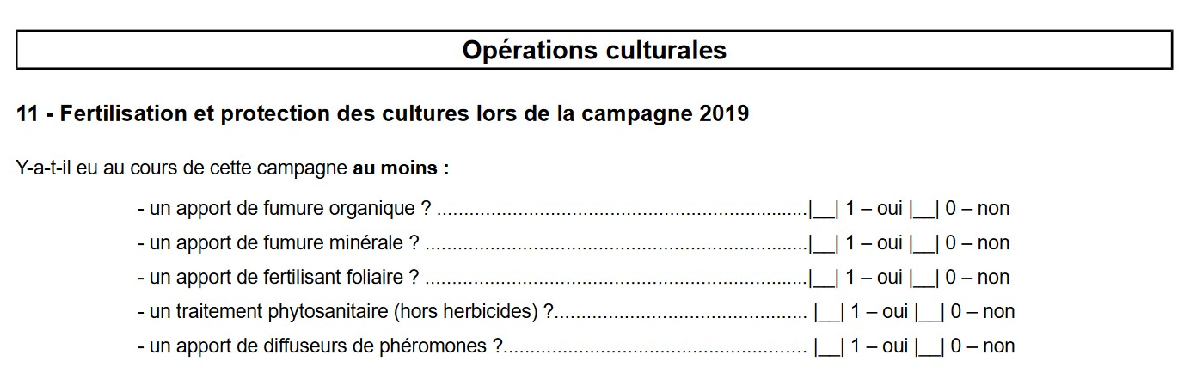
\includegraphics[scale=0.75]{figs/Chap3/PK1.pdf}
    \caption{Question extracted from the 2019 survey destined to vitivulture. The question asked is about the fertilization and protection of the crops and the use of any phyto-sanitary product.}
    \label{fig:PK1}
\end{figure}

\subsubsection{Substances sales databank}

The use of a substance can also be indirectly seen in the sales data of crop protection products. The National Bank for the Sale of Pesticides by Authorized Distributors (NBSD) \cite{BNVD} lists and archives all such data. For the same reasons of anonymity, geographically fine resolution information is not available. The most accurate resolution corresponds to postal codes. It is the same for the temporal resolution that is not finer than the yearly resolution. Rhis data set does not indicate the location and date of use of the substance. A purchaser may well be in a different location than the place of use of the substance they just purchased. Nevertheless, sales give a general indication of the intensity of use of a substance. A sudden increase in sales of a product may mean that its use is increasing in that area.  

\begin{table}[ht]\label{tab:bnvd}
\centering
\begin{tabular}{rlllrr}
  \hline
 & Year & Department & Substance & Quantity sold (in kg) & Annual rank \\ 
  \hline
1 & 2008 & INDRE & 2,4-db & 27.00 & 155 \\ 
  2 & 2009 & INDRE & 2,4-db & 24.00 & 162 \\ 
  3 & 2010 & INDRE & 2,4-db & 24.00 & 166 \\ 
  4 & 2011 & INDRE & 2,4-db & 68.00 & 148 \\ 
  5 & 2012 & INDRE & 2,4-db & 7.00 & 195 \\ 
  6 & 2013 & INDRE & 2,4-db & 72.00 & 157 \\ 
  7 & 2014 & INDRE & 2,4-db & 120.00 & 125 \\ 
  8 & 2015 & INDRE & 2,4-db & 84.00 & 146 \\ 
  9 & 2016 & INDRE & 2,4-db & 195.00 & 108 \\ 
  10 & 2017 & INDRE & 2,4-db & 348.00 & 105 \\ 
   \hline
\end{tabular}
   \caption{Annual sales of the weed killer 2,4-db in the Indre department. The last column indicates the national annual rank of the substance sales.}
\end{table}

\subsubsection{Crops cartography}

Specific pest species can be observed for each crop type. Mapping the crop types in an area can therefore provide a preliminary idea of the areas and periods of application of the substance being monitored. Some of this information is available in the graphical land register (GLR) \cite{RPG}. This database corresponds to the application forms used by farmers to obtain financial aid under the Common Agricultural Policy of the European Union (CAP). To be eligible for these grants, the crops grown on the plots must be declared. This dataset is a partial information, since asking for CAP funds is not mandatory. Therefore, the owners of the crops who have not applied for aid are not present in the database. Moreover, this register is renewed every year. It is possible that the information for certain parcels is not included in all annual editions of the GLR. Crops maps of barley and wheat are diplayed in Figure \ref{fig:crops} of Annex \ref{annex:chap:5}.

%\footnote{Available at : \url{https://www.data.gouv.fr/fr/datasets/registre-parcellaire-graphique-rpg-contours-des-parcelles-et-ilots-culturaux-et-leur-groupe-de-cultures-majoritaire/}.}

\subsubsection{Adverse effects databases}

The last example of data that can highlight clues of a substance usage are the databases for monitoring potential adverse events. They consist in medical registries providing informations on human and animal health.  
For human health, several information sources can be cited: 
\begin{itemize}
\item the Phytattitude network was developed by the Mutual Agricultural Health Insurers (MSAs). It is a network where any professional who comes into contact with phytosanitary products can indicate if he/she has health problems. This organization collects data through spontaneous reports from agricultural actors or during scheduled visits by nurses or doctors.
\item the medical-administrative databases of the MSA. They collect information on farmers' health care reimbursements.
\item the poison control centers are involved in adverse effect surveillance. They provide toxicovigilance information on toxicovigilance for the entire population. Much information about acute health problems comes up through these information channels.
\item the National network of vigilance and prevention of professional pathologies (RNV3P), whose role is to identify emerging or re-emerging occupational health risks constitutes a good source for chronic health problems.
\item the AGRICAN cohort (AGRIculture and CANcer) of the François Baclesse Center is used to measure the health status of the agricultural population compared to the general population (especially in terms of cancer burden).
\end{itemize}

Regarding animal health, INRAE provides a database on veterinary toxicovigilance (GIS Toxinelle), and the Biodiversity French Office (OFB) on wildlife toxicovigilance of wildlife. The Department of Agriculture provides additional information, such as acute mortality in bees, and its 500 ENI biovigilance program is also part of the available databases. This is a program to monitor the impact of agricultural practices on biodiversity.

\section{Example of additional useful data}\label{chp:2:4}

We discussed in Section \ref{chp:2:2} the exposure factor in monitoring a health risk. Exposure includes the ways in which the population may come into contact with the substance. The environment has a major influence on how exposure can occur. Therefore, it is important to include environmental information in the monitoring system. Since an exhaustive list of all possible data sets would prove lengthy, this section provides examples of interesting additional data sets for surface water and air quality monitoring.

\subsection{Surface water quality}

In surface water quality monitoring, stations are positionned on streams of water or lakes.  Their precise GPS location can bring insight on how a substance could diffuse once introduced into the surface water system. This information is made available by the National Institute of Geographic and Forest Information (IGN) services in the BDTOPO database. Figure \ref{fig:esu_ex} displays the river system of the Centre-Val de Loire French region with the positions of all stations. With this information at hand, stations concentrations can be directly compared according to their distance in the river system.     

\begin{figure}[ht]
    \centering
    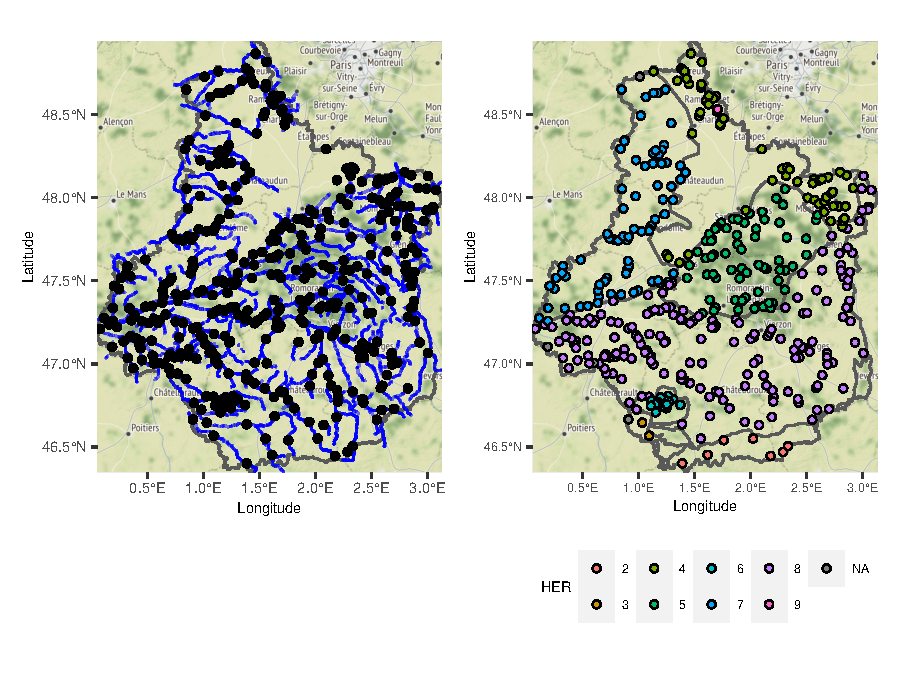
\includegraphics{Chap3/ESU_EX.pdf}
    \caption{Stations monitoring water suface in the Centre-Val de Loire french region. Two different geographical resolutions are represented. The underlying hydrographic network linking all stations is plotted on the left, the stations are colored according to their hydroecoregion on the right.}
    \label{fig:esu_ex}
\end{figure}

However, we mentionned in Section \ref{chp:2:3} that an individual station does not provide much measurments. Therefore, to derive information from these data, one can work on a different resolution than that of the station.  Thus, there is a trade-off between the number of data available to make a statistical statement about a spatial area and the spatial resolution accuracy. Another interesting level of resolution that was briefly mentionned in Section \ref{chp:2:2} are the hydro-ecoregions (HER). They are geographic units in which hydrographic ecosystems share common characteristics. The criteria by which they are delineated combine characteristics of geology, terrain, and climate \cite{wasson:hal-02580774}. INRAE services provides such information. Pooling all samples from the HERs can provide a satisfactory level of aggregation but it would be at the expense of the spatial resolution. Figure \ref{fig:esu_ex} shows how the stations are distributed in the HER.  

\subsection{Air quality}

Meteorological data is an important data set for monitoring air quality, especially any information that can be found about wind (wind direction, wind strength, etc.). Historical weather records are now available as open data on the Météo France website \cite{SYNOP}. Figure \ref{fig:air_ex} illustrates the cross-referencing of data from air quality monitoring stations with meteorological data. Note that in this example we chose to represent stations within the study region, but information from outlying areas can also provide interesting informations on air pollution in the selected area. This example also shows that concentration monitoring tasks depend on the application context. The coherence of any data set included in the analysis must be discussed.   

\begin{figure}[ht]
    \centering
    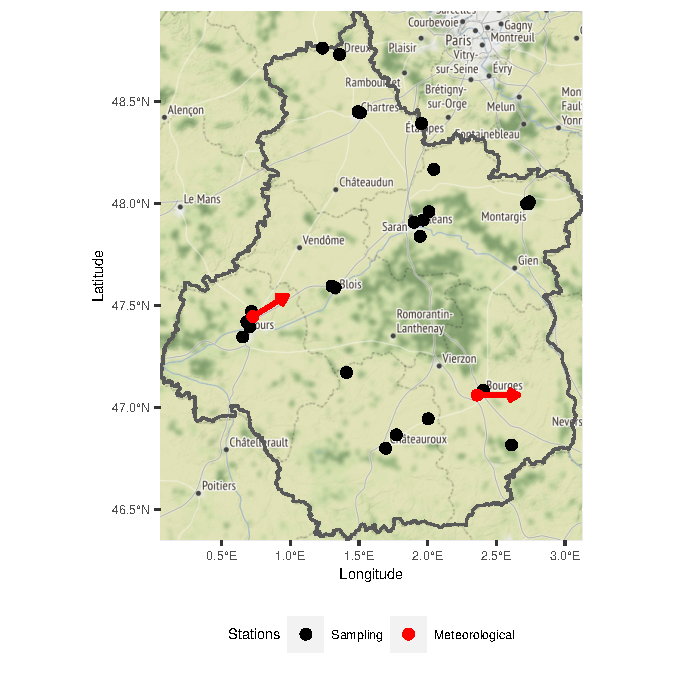
\includegraphics{Chap3/AIR_EX_DATA.pdf}
    \caption{All active stations measuring air quality on March the 1st of 2021 coupled with meteorological stations active that day. The main wind direction and speed measured that day is mapped with the red arrows.}
    \label{fig:air_ex}
\end{figure}

\section{Surveillance of pesticides data}\label{chp:2:5}

This section proposes an initial exploratory approach to monitoring pesticide concentrations using data from Sections \ref{chp:2:3} and \ref{chp:2:4}. The goals set in \ref{chp:2:2} may be difficult to achieve because of the specific French administrative organization discussed in \ref{chp:2:1}. The spatiotemporal nature of concentration data requires appropriate techniques for their representation, which were reviewed in \cite{Andrienko2003,cressie2015,Maimon2010}. As mentioned in \cite{Ansari2019}, spatial and temporal resolution is a key factor in the analysis and cannot be chosen automatically. Performing proper analysis of concentration data requires the involvement of domain. experts. This includes the development of visualization tools. Several methods are available for visualizing spatiotemporal data. This section presents some visualization techniques and discusses their limitations.

The spatial map plots or iterative maps \cite{Andrienko2003} are an effective way to extract information from these data. They consist of maps of the same phenomenon at different times, as in Figure \ref{fig:spa_ex}. There is a clear seasonal pattern in this figure. We can conclude that prosulfocarb is applied in autumn, and this information is confirmed by the crops targeted by this substance, namely winter wheat crops. The two years of observation were segmented by the choice of temporal resolution of the seasons. Although this is a coherent choice, it has some limitations. For example, it cannot account for years in which treatment started earlier or later due to climatic conditions. In addition, it cannot help to determine precisely the nature of the temporal change in the signal. Only the summary indicator of quantification rate is used. Nothing is known about the maximum or average concentrations.
 
\begin{figure}[ht]
    \centering
    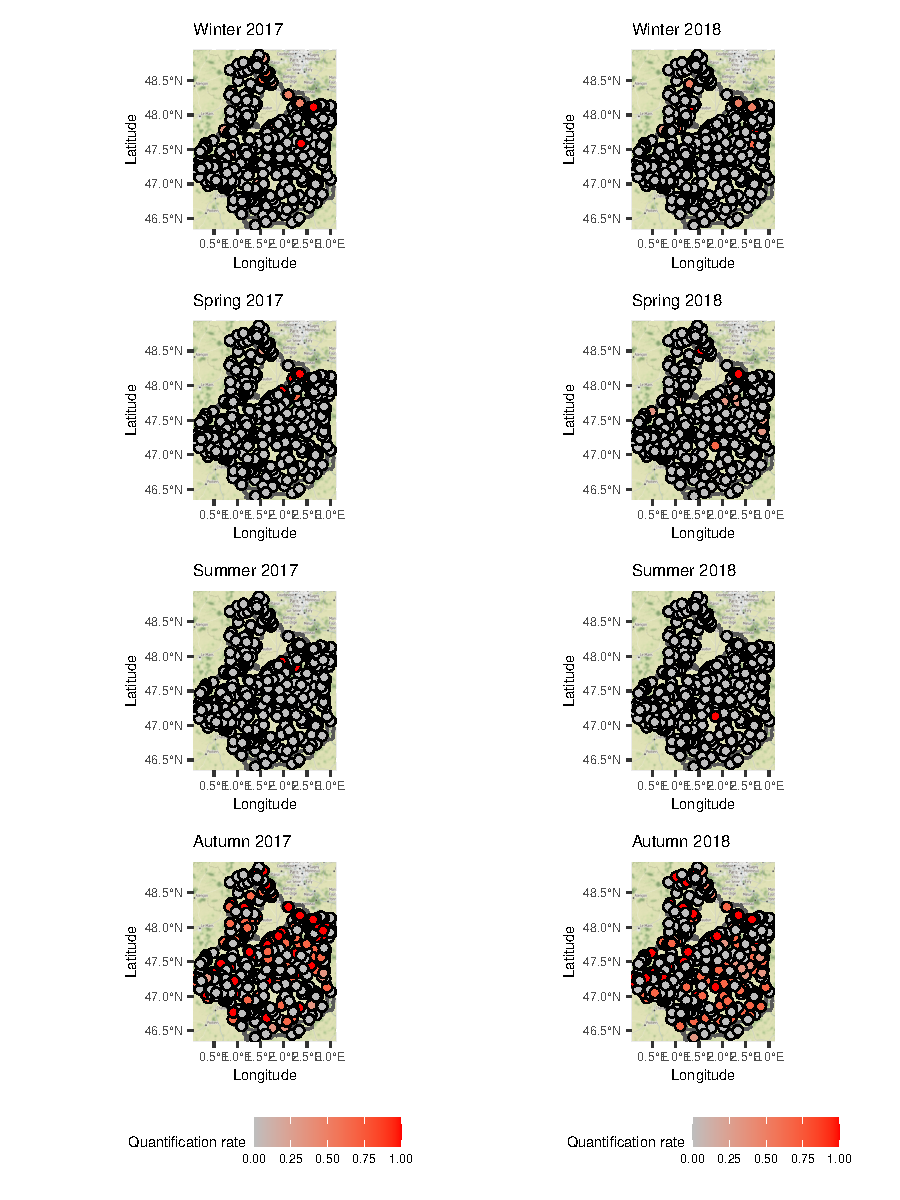
\includegraphics{Chap3/Spatial_maps.pdf}
    \caption{Spatial maps in time. Prosulfocarbe's quantification rate of each station was computed for each season of 2017 and 2018.}
    \label{fig:spa_ex}
\end{figure}

Another conventional representation is the display of information with a map animation \cite{Andrienko2003}. In this method, the information displayed on the computer screen is updated depending on the selected spatial area. Figure \ref{fig:tsplot_ex} shows a practical example of this technique. Concentrations of prosulfocarbe in the Centre-Val de Loire French region of France are displayed according to the selected HER region. Two limitations arise with this visualization. The first is the choice of spatial resolution. The HER were chosen to cluster the geography of the region. However, it can be seen that these can be very large regions. Stations located at opposite corners of a single HER may not have similar concentration values. Spatial heterogeneity of agricultural practices may occur at finer resolution. HER may not accurately capture regions where concentrations are homogeneously distributed. We will show how we deal with spatial resolution in Chapter \ref{chp:5}. This presentation also raises the question of the choice of temporal resolution. All samples available in the study period are shown in Figure \ref{fig:tsplot_ex}. There is a clear break in the three series around 2015. There appears to be a change in concentration regimes. A finer temporal resolution combined with a comparison based on statistical inference of the selected geographic regions could better help experts in the interpretation. Chapters \ref{chp:3} and \ref{chp:4} will address the issue of temporal resolution.

\begin{figure}[ht]
    \centering
    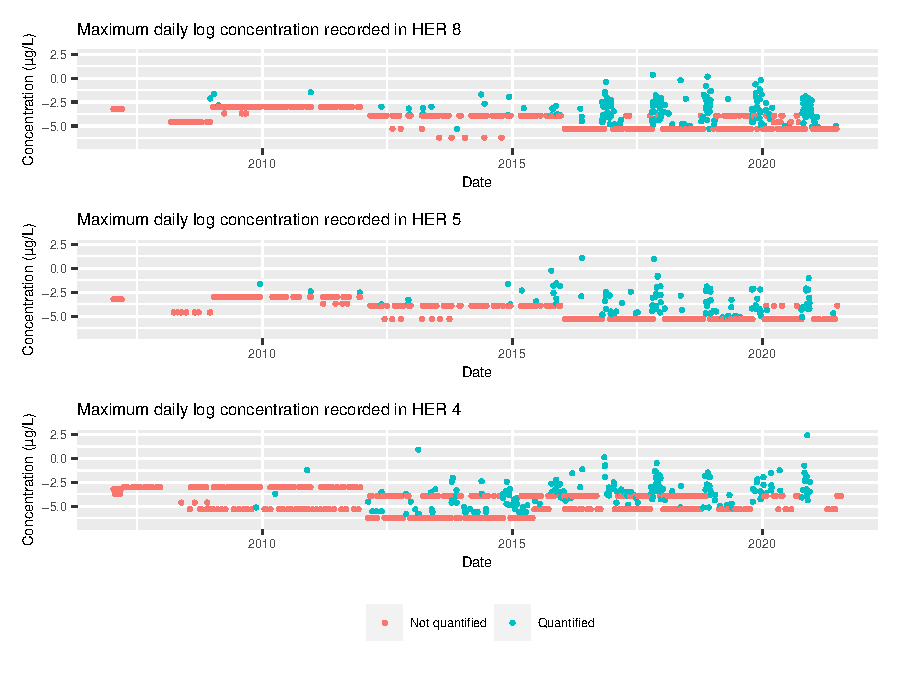
\includegraphics{Chap3/TS_plot.pdf}
    \caption{Time series plot of HER 8,5 and 4 daily maximum concentrations. The log scale was used for a easier visualization.}
    \label{fig:tsplot_ex}
\end{figure}




%The minimum number of dimensions to describe them is three: two for space as a pair of longitudes and latitudes; one for time. \cite{cressie2015} presents in his book several methods of descriptive statistics for the representation of such data. The most intuitive method to plot spatiotemporal data are marginal and conditional plot. There are several ways to make them.

 
%\begin{figure}[ht]
%    \centering
%    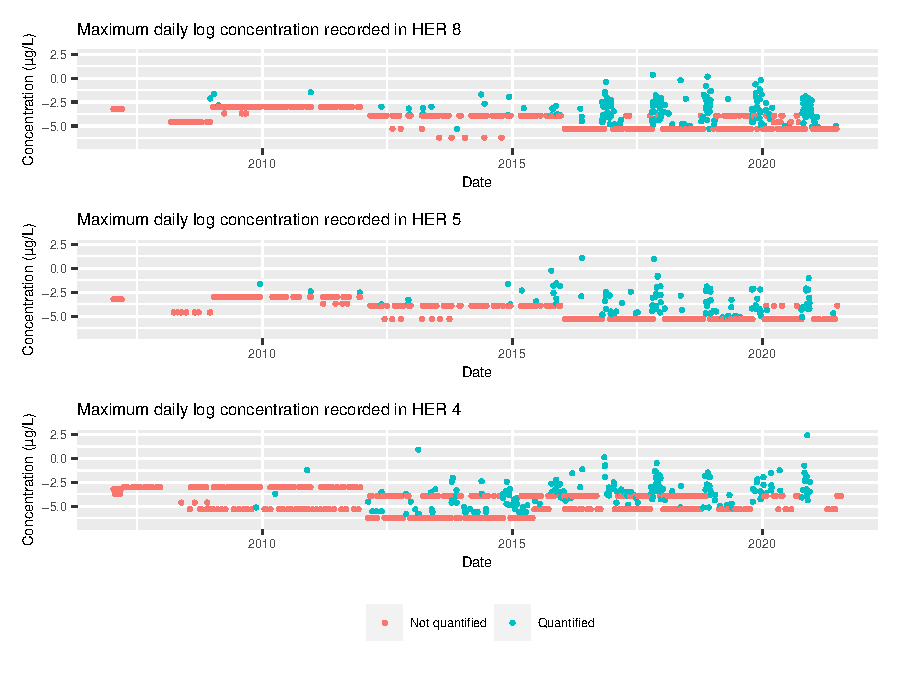
\includegraphics{Chap3/TS_plot.pdf}
%    \caption{Time series plot of HER 8,5 and 4 daily maximum concentrations. The log scale was used for a easier visualization.}
%    \label{fig:tsplot_ex}
%\end{figure}
 


%Another example of representation is the \textbf{space (1-D)/time plots} shown in Figure \ref{fig:S1Dplot}. It consists in fixing a dimension in space whether longitude or latitude and to plot some indicators summarised on that dimension against time. In Figure \ref{fig:S1Dplot}, the longitude was cut into regular intervals and time was segmented in seasons. The plot shows once again a very clear temporal seasons that appears in time in the region. The location of those changes are not clearly displayed by those plots though. We are not able to determine if the large quantification rates are in the central areas of the region or not (given that we miss the latitude information). Although those plots provide an excellent first overview and can help to quickly understand the structure under spatiotemporal data, it does not provide sufficient precision to localize in space and time some interesting signals.    

%\begin{figure}[ht]
%    \centering
%    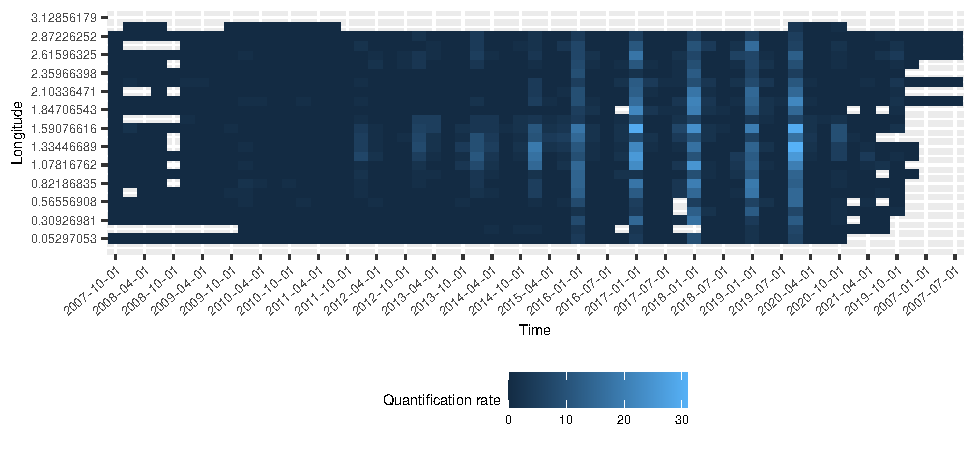
\includegraphics{Chap3/T1Dplot.pdf}
%    \caption{Space (1-D)/Time plots. Grey tiles correspond to location and moment were no sample were collected.}
%    \label{fig:S1Dplot}
%\end{figure}

%All of those representation methods can't capture all the information carried by the data set. We propose to handle it in a dynamic way using the application environment R-shiny. Integrating dynamic response to a user's requests is an efficient way to combine a descriptive view with models results. The application overview will be given in section 6.